\pdfoutput=1
\documentclass[twocolumn]{aastex62}
%%\documentclass[]{emulateapj}

%Accepted/received/... %%

\received{xxx}
\revised{yyy}
\accepted{zzz}

%% Command to document which AAS Journal the manuscript was submitted to.
\submitjournal{AAS Journals}

%% Short title/authors

\shorttitle{LXUV History of TRAPPIST-1}
\shortauthors{Fleming et al.}

%% Begin document, title, packages %%
\usepackage{hyperref}
\usepackage{xspace}
\usepackage{graphicx}
\usepackage{amsmath}
\usepackage[caption=false]{subfig}

%% Custom commands
\def\mearth{{\rm\,M_\oplus}}
\def\rearth{{\rm\,R_\oplus}}
\def\msun{{\rm\,M_\odot}}
\def\rsun{{\rm\,R_\odot}}
\def\lsun{{\rm\,L_\odot}}
\def\gsim{~\rlap{$>$}{\lower 1.0ex\hbox{$\sim$}}}
\def\lsim{~\rlap{$<$}{\lower 1.0ex\hbox{$\sim$}}}

\newcommand{\xxx}[1]{{\textbf{#1}}}
\newcommand{\vplanet}[0]{\texttt{VPLanet}\xspace}
\newcommand{\emcee}[0]{\texttt{emcee}\xspace}
\newcommand{\approxposterior}[0]{\texttt{approxposterior}\xspace}
\newcommand{\eqtide}[0]{\texttt{EQTIDE}\xspace}
\newcommand{\stellar}[0]{\texttt{STELLAR}\xspace}
\newcommand{\kepler}[0]{\textit{Kepler}\xspace}
\newcommand{\jwst}[0]{\textit{JWST}\xspace}

%% Begin doc %%
\begin{document}

\title{On The XUV Luminosity Evolution of TRAPPIST-1}

%% AUTHORS %%

%%\correspondingauthor{David P. Fleming}
%%\email{dflemin3@uw.edu}

%%\author[0000-0001-9293-4043]{David P. Fleming}
\author[0000-0001-9293-4043]{David P. Fleming}
\affil{Astronomy Department, University of Washington \\
Box 951580, Seattle, WA 98195}
\affil{NASA NExSS - Virtual Planetary Laboratory Lead Team, USA}
% ORCID 0000-0001-9293-4043

\author{Rory Barnes}
\affiliation{Astronomy Department, University of Washington \\
Box 951580, Seattle, WA 98195}
\affil{NASA NExSS - Virtual Planetary Laboratory Lead Team, USA}
% no orcid

\author[0000-0002-0296-3826]{Rodrigo Luger}
\affil{NASA NExSS - Virtual Planetary Laboratory Lead Team, USA}
\affiliation{Center for Computational Astrophysics, Flatiron Institute \\
New York, NY 10010}
% ORCIF 0000-0002-0296-3826

\author[0000-0002-9623-3401]{Jacob T. VanderPlas}
\affiliation{Google \\
601 N 34th St, Seattle, WA 98103}
% ORCID 0000-0002-9623-3401

%% ABSTRACT %%

\begin{abstract}

We model the long-term XUV luminosity of TRAPPIST-1 to constrain the evolving high-energy radiation environment experienced by its planetary system. Using Markov Chain Monte Carlo (MCMC), we derive probabilistic constraints for TRAPPIST-1's stellar and XUV evolution that account for observational uncertainties, degeneracies between model parameters, and empirical data of low-mass stars. We constrain TRAPPIST-1's mass to $m_{\star} = 0.089 \pm{0.001}$ M$_{\odot}$ and find that its early XUV luminosity likely saturated at $\log_{10}(L_{XUV}/L_{bol}) = -3.05^{+0.24}_{-0.10}$. From our posterior distributions, we infer that there is a ${\sim}43\%$ chance that TRAPPIST-1 is still in the saturated phase today, suggesting that TRAPPIST-1 has maintained high activity and $L_{XUV}/L_{bol} \approx 10^{-3}$ for several Gyrs. TRAPPIST-1's planetary system therefore likely experienced a persistent and extreme XUV flux environment, potentially driving significant atmospheric erosion and volatile loss. The inner planets likely received XUV fluxes ${\sim}10^3 - 10^4\times$ that of the modern Earth during TRAPPIST-1's 1 Gyr-long pre-main sequence phase. Deriving these constraints via MCMC is computationally non-trivial, so scaling our methods to constrain the XUV evolution of a larger number of M dwarfs that harbor terrestrial exoplanets would incur significant computational expenses. We demonstrate that \approxposterior, a Python machine learning package for approximate Bayesian inference using Gaussian processes, can efficiently replicate our analysis. We find that it derives constraints that are in good agreement with our MCMC, although it underestimates the uncertainties for two parameters by $30\%$. \approxposterior requires $330\times$ less computational time than traditional MCMC methods in this case, demonstrating its utility in efficient Bayesian inference.

\end{abstract}

%% Keywords %%

\keywords{}

%% Intro %%

\section{Introduction} \label{sec:intro}

The James Webb Space Telescope (JWST) is poised to detect and characterize the first terrestrial exoplanet atmospheres via transmission spectroscopy. This search will likely focus on planets orbiting nearby M dwarfs given their favorable relative transit depths, the potential buildup of biosignature gases due to UV-driven photochemisty \citep{Segura2005}, and the large occurrence rates of M dwarf planets \citep{Dressing2015}. The correct interpretation of those observations, however, is predicated on understanding the system's long-term evolution, most importantly processes that could impact the planet's atmospheric state and habitability, such as atmospheric escape, water loss, and the potential buildup of an abiotic O$_2$ atmosphere \citep{Watson1981,Lammer2003,MurrayClay2009,Luger2015}. These volatile escape mechanisms are partially driven by the host star's XUV luminosity (X-ray and EUV emission ranging over approximately 1-1000\AA), and therefore characterizing the long-term stellar XUV evolution of late M-dwarfs is critical to assessing the present state of their planets, including habitability.

High-energy stellar radiation originates from the corona via the heating of magnetically-confined plasma \citep{Vaiana1981}. The stellar magnetic field is likely generated via differential rotation within the stellar convective envelope \citep{Parker1955}, linking rotation to stellar activity and XUV emission. Stellar rotation rates slow over time due to magnetic braking \citep{Skumanich1972}, causing XUV emission to decline with time. The X-ray luminosity ($L_{X}$) of FGK stars, for example, has been empirically shown to monotonically decrease with age \citep{Jackson2012}. This trend has also been observed for commonly-used proxies for stellar age, rotation period and Rossby number \citep[Ro = $P_{rot}/\tau$ for convective turnover timescale $\tau$,][]{Pizzolato2003,Wright2011}. Stellar activity evolution is characterized by two distinct phases. First, in the saturated phase, young, rapidly-rotating stars ($\mathrm{Ro}\lsim 0.1$) maintain a constant $L_{X}/L_{bol} \approx 10^{-3}$ \citep{Wright2011,Jackson2012}. Then, at longer rotation periods and larger Ro, stars transition to the unsaturated phase in which $L_{X}/L_{bol}$ exponentially decays over time \citep{Pizzolato2003,Ribas2005}. Recent work has shown that the stellar dynamo processes that generate magnetic fields and drive XUV emission in fully-convective M dwarfs follow the same evolution with Ro as described above for solar-type stars \citep{Wright2016,Wright2018}. We can therefore apply this model to examine the XUV evolution of individual fully-convective stars.

TRAPPIST-1 \citep{Gillon2016,Gillon2017}, an ultracool dwarf located 12 pc from Earth, harbors 7 approximately Earth-sized transiting planets that are prime targets for JWST transmission spectroscopy observations \citep{Morley2017,Lincowski2018,Lustig2019}. TRAPPIST-1's high observed L$_{X}$ \citep{Wheatley2017}, short photometric rotation period \citep[3.3 d, ][]{Luger2017}, and low Rossby number \citep[Ro $\approx 0.01$, ][]{Roettenbacher2017} suggest that TRAPPIST-1 is still saturated today \citep{Pizzolato2003,Wright2011,Wright2018}. Both \citet{Roettenbacher2017} and \citet{Morris2018} suggest that the photometrically-determined rotation period is inaccurate, with the latter study proposing that the 3.3 d period corresponds to a characteristic timescale for active regions on the stellar surface. TRAPPIST-1's $v \sin i = 6$ km s$^{-1}$ \citep{Barnes2014}, however, implies a rotation period of $\approx 1$ d for $i = 90^{\circ}$, providing evidence that TRAPPIST-1's rapid rotation is physical and consistent with saturation \citep[$P_{rot} \lsim 20$ d,][]{Wright2018}. The TRAPPIST-1 planetary system currently receives significant high-energy fluxes \citep{Bourrier2017b,Wheatley2017,Peacock2019}, possibly a consequence of TRAPPIST-1 remaining in the saturated regime. These fluxes were likely more extreme during the pre-main sequence, driving significant water loss and potentially rendering the planets uninhabitable \citep{Bolmont2017,Bourrier2017a}. 

Here, we model the long-term stellar and XUV evolution of TRAPPIST-1 to characterize the evolving XUV environment of its planetary system. We use MCMC to derive probability distributions for our model parameters that describe the XUV evolution and are consistent with TRAPPIST-1's observed properties and their uncertainties. TRAPPIST-1 is not the only system that merits this modelling, however, as the Transiting Exoplanet Survey Satellite will likely discover additional transiting planets orbiting in the habitable zone of nearby M dwarfs \citep{Barclay2018}, some of which will likely be suitable targets for atmospheric characterization with JWST. 

In this work, we show that stellar XUV histories can be accurately inferred using machine learning \citep[\approxposterior, ][]{FlemingVanderPlas2018}, but using $330\times$ less computational resources than traditional MCMC methods. This massive speed-up enables our methods to scale to additional stars that host potential targets for atmospheric characterization. 

We describe our model and statistical methods in $\S$~\ref{sec:methods} and $\S$~\ref{sec:mcmc}, respectively. We present our results in $\S$~\ref{sec:results}, demonstrate the ability of machine learning to reproduce our analysis in $\S$~\ref{sec:approx}, and discuss the implications of our results in $\S$~\ref{sec:discussion}.

% extra
% , so their dynamos likely differ, e.g. magnetic field generation via convective turbulence \citep{Dobler2006} rather than the tachocline-driven generation theorized for late-type stars with radiative cores \citep{Durney1993}. 

\section{Methods} \label{sec:methods}

\subsection{XUV Evolution} \label{sec:model}

We simulate TRAPPIST-1's stellar evolution using the \stellar module in \vplanet\footnote{\vplanet is publicly available at \href{https://github.com/VirtualPlanetaryLaboratory/vplanet}{https://github.com/VirtualPlanetaryLaboratory/vplanet}.} \citep{Barnes2019}, which performs a bicubic interpolation over mass and age of the \citet{Baraffe2015} stellar evolution tracks. The \citet{Baraffe2015} models (also employed by both \citet{Burgasser2017} and \citet{vanGrootel2018} to constrain TRAPPIST-1's stellar properties) were computed for solar metallicity stars and hence are suitable for TRAPPIST-1 whose [Fe/H] is consistent with solar \citep{Gillon2016}, although \citet{Burgasser2017} argue TRAPPIST-1 has a slightly super-solar metallicity based on isochrone modeling.

The X-ray luminosity, L$_{X}$, evolution of fully-convective stars follows the same broken power law model examined for partially-convective FGK stars \citep{Wright2016,Wright2018}. We assume TRAPPIST-1's L$_{XUV}$ evolution traces that of L$_{X}$ and use the model of \citet{Ribas2005},
\begin{align}
\label{eqn:lxuv}
\frac{L_\mathrm{XUV}}{L_\mathrm{bol}} = \left\{
				\begin{array}{lcr}
					f_\mathrm{sat} &\ & t \leq t_\mathrm{sat} \\
					f_\mathrm{sat}\left(\frac{t}{t_\mathrm{sat}}\right)^{-\beta_\mathrm{XUV}} &\ & t > t_\mathrm{sat}
				\end{array}
				\right.,
\end{align}
where $f_{sat}$ is the constant ratio of stellar XUV to bolometric luminosity during the saturated phase, $t_{sat}$ is the duration of the saturated phase, and $\beta_{XUV}$ is the exponent that controls how steeply L$_{XUV}$ decays after saturation. 

\subsection{Markov Chain Monte Carlo} \label{sec:mcmc}

We use \texttt{emcee}, a Python implementation of the affine-invariant Metropolis-Hastings MCMC sampling algorithm \citep{ForemanMackey2013}, to infer posterior probability distributions for our model parameters. These distributions are conditioned on observations of TRAPPIST-1 and the activity evolution of late-type stars and account for both observational uncertainties and correlations between parameters. Our model parameters that we fit for via MCMC comprise the state vector
\begin{equation} \label{eqn:state}
    \textbf{x} = \{m_{\star}, f_{sat}, t_{sat}, \mathrm{age}, \beta_{XUV}\},
\end{equation}
where $m_{\star}$ and age are the stellar mass and age, respectively, and the other parameters are defined by Eqn.~\ref{eqn:lxuv}. All of the code used to perform the simulations and analysis in this work is publicly available online.\footnote{ \href{https://github.com/dflemin3/trappist}{https://github.com/dflemin3/trappist}}

\subsection{Priors} \label{sec:mcmc:priors}

Since we have few available observable properties of TRAPPIST-1 to use to condition our analysis ($L_{bol}$ and $L_{XUV}$, see $\S$~\ref{sec:mcmc:like}), our prior probability distributions will strongly impact our results. We use previous studies and empirical data of late M dwarfs to assemble the best available constraints to serve as priors for our MCMC analysis. Following \citet{vanGrootel2018}, we rely on TRAPPIST-1's luminosity and age to constrain its mass. We therefore adopt a simple uniform prior of $m_{\star} \sim \mathcal{U}(0.07, 0.11)$. For the age, we use the empirical estimate for TRAPPIST-1 derived by \citet{Burgasser2017}, age $\sim \mathcal{N}(7.6, 2.2^2)$ Gyr, as their thorough analysis considered both observations of TRAPPIST-1 and a host of empirical age indicators for ultracool dwarfs. We cap the maximum age we consider at 12 Gyr. Younger ages have been suggested based on TRAPPIST-1's activity \citep[e.g.~$\gsim 500$ Myr,][]{Bourrier2017b}, but here we argue that behavior is consistent with an extended saturation timescale.

We construct an empirical $f_{sat} = \log_{10}(L_{XUV}/L_{bol})$ distribution from the sample of fully-convective, saturated M dwarfs with observed $L_{X}$ from \citet{Wright2011}. For each star in the \citet{Wright2011} sample, we follow \citet{Wheatley2017} and estimate $L_{XUV}$ as a function of L$_{X}$ using Eqn.~(2) from \citet{Chadney2015}. We find that the distribution is well-approximated by a normal distribution, $f_{sat} \sim \mathcal{N}(-2.92, 0.26^2)$, and we adopt it as our prior.  

The duration of the saturated phase is estimated to be $t_{sat} \approx 100$ Myr for FGK stars \citep{Jackson2012}. Studies of stellar activity of late type stars as a function of stellar age, or its proxy, rotation period, indicate that the activity lifetime, and hence duration of the saturated phase, is likely longer for later-type stars \citep{Shkolnik2014,Wright2011,West2015}, with fully-convective M dwarfs potentially remaining active throughout their lifetimes \citep[$t_{sat} \gsim 7$ Gyr,][]{West2008,Schneider2018}. Furthermore, the spin-down timescales of late M dwarfs increases with decreasing stellar mass \citep{Delfosse1998}, with late M dwarfs retaining rapid rotation longer than earlier-type stars and hence remaining active for up to $P_{rot} \approx 86$ d \citep{West2015}, well-beyond TRAPPIST-1's estimated rotation period. Given these constraints, we adopt a broad uniform $t_{sat}$ prior distribution capped by the maximum age we consider, $t_{sat} \sim \mathcal{U}(0.1, 12)$ Gyr. 

In the unsaturated phase, $L_{X}$, and hence $L_{XUV}$, decay exponentially with powerlaw slope $\beta_{XUV}$ \citep{Ribas2005}. \citet{Jackson2012} find that $\beta_{XUV}$ does not significantly vary with stellar mass in their sample of FGK stars. Since \citet{Wright2016} found that the X-ray evolution of fully-convective stars is qualitatively similar to that of partially-convective FGK stars, we adopt the $\beta_{XUV}$ distribution of late K dwarfs from the \citet{Jackson2012} sample as our prior, $\beta_{XUV} \sim \mathcal{N}(-1.18, 0.31^2)$.

%\begin{deluxetable}{lcc}
%\tabletypesize{\small}
%\tablecaption{Prior Distributions \label{tab:priors}}
%\tablewidth{0pt}
%\tablehead{
%\colhead{Parameter [units]} & \colhead{Prior} & \colhead{Notes}
%}
%\startdata
%$m_\star$ [$M_{\odot}$] & $\mathcal{U}(0.07, 0.11)$ & -- \\  
%$f_{sat}$ & $\mathcal{N}(-2.92, 0.26^2)$ & \citet{Wright2011}  \\
%$t_{sat}$ [Gyr] & $\mathcal{U}(0.1, 12)$ & -- \\
%age [Gyr] & $\mathcal{N}(7.6, 2.2^2)$ & \citet{Burgasser2017} \\
%$\beta_{XUV}$ & $\mathcal{N}(-1.18, 0.31^2)$ & \citet{Jackson2012}
%\enddata \vspace*{0.1in}
%\end{deluxetable}

\subsection{Likelihood Function and Convergence} \label{sec:mcmc:like}

We further condition our analysis on TRAPPIST-1's observed bolometric luminosity, $L_{bol} = 5.22 \pm{0.19} \times 10^{-4} \ L_{\odot}$ \citep{vanGrootel2018}, and $L_{XUV}/L_{bol}$ \citep{Wheatley2017}. We convolve the \citet{vanGrootel2018} $L_{bol}$ measurement with the $L_{XUV}/L_{bol}$ constraints from \citet{Wheatley2017}, finding $L_{XUV} = 3.9 \pm{0.5} \times 10^{-7} \ L_{\odot}$ today.

For a given state vector \textbf{x}, we define our likelihood function, $\mathcal{L}$, as
\small
\begin{equation} \label{eqn:lnlike}
    \ln \mathcal{L} \propto -\frac{1}{2} \left[ \frac{(L_{bol} - L_{bol}(\textbf{x}))^2}{\sigma_{L_{bol}}^2} + \frac{(L_{XUV} - L_{XUV}(\textbf{x}))^2}{\sigma_{L_{XUV}}^2} \right] \\
\end{equation}
\normalsize
where $L_{bol}$, $L_{XUV}$ and $L_{bol}(\textbf{x})$, $L_{XUV}(\textbf{x})$ are the observed values and \vplanet outputs given \textbf{x}, respectively and $\sigma_{L_{bol}}$ and $\sigma_{L_{XUV}}$ are the observational uncertainties. We compute the total logprobability for each \textbf{x} by summing $\mathcal{L}$ and $\ln \mathrm{Prior}(\textbf{x})$, the log prior probability of \textbf{x}. We compute the log prior using the distributions described in $\S$~\ref{sec:mcmc:priors}. 

We run our MCMC with 100 parallel chains for 10,000 iterations, initializing each chain by randomly sampling each element of \textbf{x} from their respective prior distributions. During each step of the MCMC chain, \vplanet takes \textbf{x} as input and simulates TRAPPIST-1's evolution up to the age in \textbf{x}, predicting $L_{bol}$ and $L_{XUV}$ to evaluate the likelihood function. We discard the first 500 iterations as burn-in and assess the convergence of our MCMC chains by computing the integrated autocorrelation length and acceptance fraction for each chain. We find a mean acceptance fraction of 0.45 and a minimum and mean number of iterations per integrated autocorrelation length of 75 and 110, respectively, indicating that our chains have converged \citep{ForemanMackey2013}. Given our integrated autocorrelation lengths, our MCMC chain yielded about 10,000 effective samples from the posterior distribution.

\subsection{Inference with \approxposterior} \label{sec:methods:approx}

The methods presented above can be applied to any late-type star to constrain its $L_{XUV}$ history, given suitable priors and observational constraints. Our MCMC analysis, however, required 3,700 core hours on the University of Washington Hyak supercomputer to converge. The main computational cost is incurred by running a $10$~s \vplanet simulation each MCMC step to evaluate the likelihood, requiring ${\sim}1,000,000$ simulations in total for the full MCMC. Assuming similar convergence properties, repeating this analysis for even a modest sample of 30 stars would require~${\sim} 110,000$ core-hours, a significant computational expense. Moreover, performing a similar analysis with a more computationally-expensive model, perhaps one that interpolates stellar models over metallicity to additionally fit for [Fe/H], would only exacerbate this issue.

We apply \approxposterior\footnote{\approxposterior is publicly available at \href{https://github.com/dflemin3/approxposterior}{https://github.com/dflemin3/approxposterior}.}, an open source Python machine learning package \citep{FlemingVanderPlas2018}, to compute an accurate approximation to the true MCMC-derived posterior distribution for TRAPPIST-1's XUV evolution, while minimizing the computational cost. \approxposterior, an implementation of the ``Bayesian Active Learning for Posterior Estimation" (BAPE) algorithm of \citet{Kandasamy2015}, trains a Gaussian process (GP) surrogate for the likelihood evaluation, learning on the results of \vplanet simulations. The GP is then used within an MCMC sampling algorithm, e.g. \emcee, to quickly obtain the posterior distribution. In our case, predicting the likelihood using the GP (${\sim} 130 \mu$s) is $80,000 \times$ faster than running \vplanet (10s) each likelihood evaluation, yielding a massive reduction in computational cost.

Following \citet{Kandasamy2015}, \approxposterior iteratively improves the GP's predictive ability by identifying high-likelihood regions in parameter space where the GP predictions are uncertain. \approxposterior then evaluates \vplanet in those regions to supplement the training set, improving the GP's predictive ability in the relevant regions of parameter space, while minimizing the number of forward model evaluations required for suitable predictive accuracy. Similar techniques using a GP surrogate model have been shown to rapidly and accurately infer Bayesian posterior distributions for computationally-expensive cosmology studies \citep[e.g.][]{Bird2019}.

To model the covariance between points in the GP training set, we use a squared exponential kernel,
\begin{equation} \label{eqn:kernel}
k(x_i, x_j) = \exp \left( - \frac{(x_i - x_j)^2}{2l^2} \right),
\end{equation}
where $x_i$ and $x_j$ are two arbitrary points in parameter space and $l$ is a hyperparameter that controls the scale length of the correlations. We assume correlations in each dimension have different scale lengths and fit for each $l$ by optimizing the GP's marginal likelihood of the training set data using the Nelder-Mead algorithm, randomly restarting this optimization 25 times to mitigate the influence of local extrema. We run \approxposterior for 10 iterations, initially training the GP on a set of 250 \vplanet simulations with initial conditions sampled from our prior distributions. For each iteration, \approxposterior selects 100 new training points, alternating between the \citet{Kandasamy2015} and \citet{Wang2017} selection criteria, both based on GP predictive uncertainty. \approxposterior runs \vplanet at each point for a total of 1,250 training samples. The trained GP is then used within \emcee to quickly obtain the approximate posterior distribution following the same procedure described in $\S$~\ref{sec:mcmc}.

%% Results %%

\section{Results} \label{sec:results}

\subsection{The Evolution of TRAPPIST-1}

In Fig.~\ref{fig:corner}, we display the posterior probability distributions for our model parameters derived via MCMC. We adopt the median values of the marginalized distributions as our best-fit solutions and derive the lower and upper uncertainties using the 16th and 84th percentiles, respectively. 

TRAPPIST-1 likely maintained a large $L_{XUV}$ throughout its lifetime as we find $f_{sat} = -3.05^{+0.24}_{-0.10}$ and $t_{sat} = 6.85^{+3.43}_{-3.15}$ Gyr, consistent with observed $L_{XUV}/L_{bol}$ and long activity lifetimes of late M dwarfs \citep{West2008,Wright2018}. The long upper-tail in the marginalized $f_{sat}$ distribution arises from the combination of the degeneracy between $f_{sat}$ and $t_{sat}$ and from our strong empirical $f_{sat}$ prior that disfavors $f_{sat} \gsim -2.5$. The degeneracy stems from our model attempting to match TRAPPIST-1's observed $L_{XUV}$. For example, larger values of $f_{sat}$ produce high initial $L_{XUV}$, requiring shorter $t_{sat}$, and hence an earlier transition to unsaturated $L_{XUV}$ decay, to decrease $L_{XUV}$ to its observed value, and vice versa. From the posterior distribution, we infer that there is a $43\%$ chance that TRAPPIST-1 is still in the high-$L_{XUV}$ saturated phase today, suggesting that the TRAPPIST-1 planets could have undergone prolonged water loss. Our analysis strongly disfavors short saturation timescales, with only a $0.4\%$ chance that $t_{sat} \leq 1$ Gyr, the saturation timescale adopted by \citet{Luger2015} in their analysis of water loss from exoplanets orbiting in the habitable zone of late M dwarfs.

\begin{figure*}[t]
\centering
	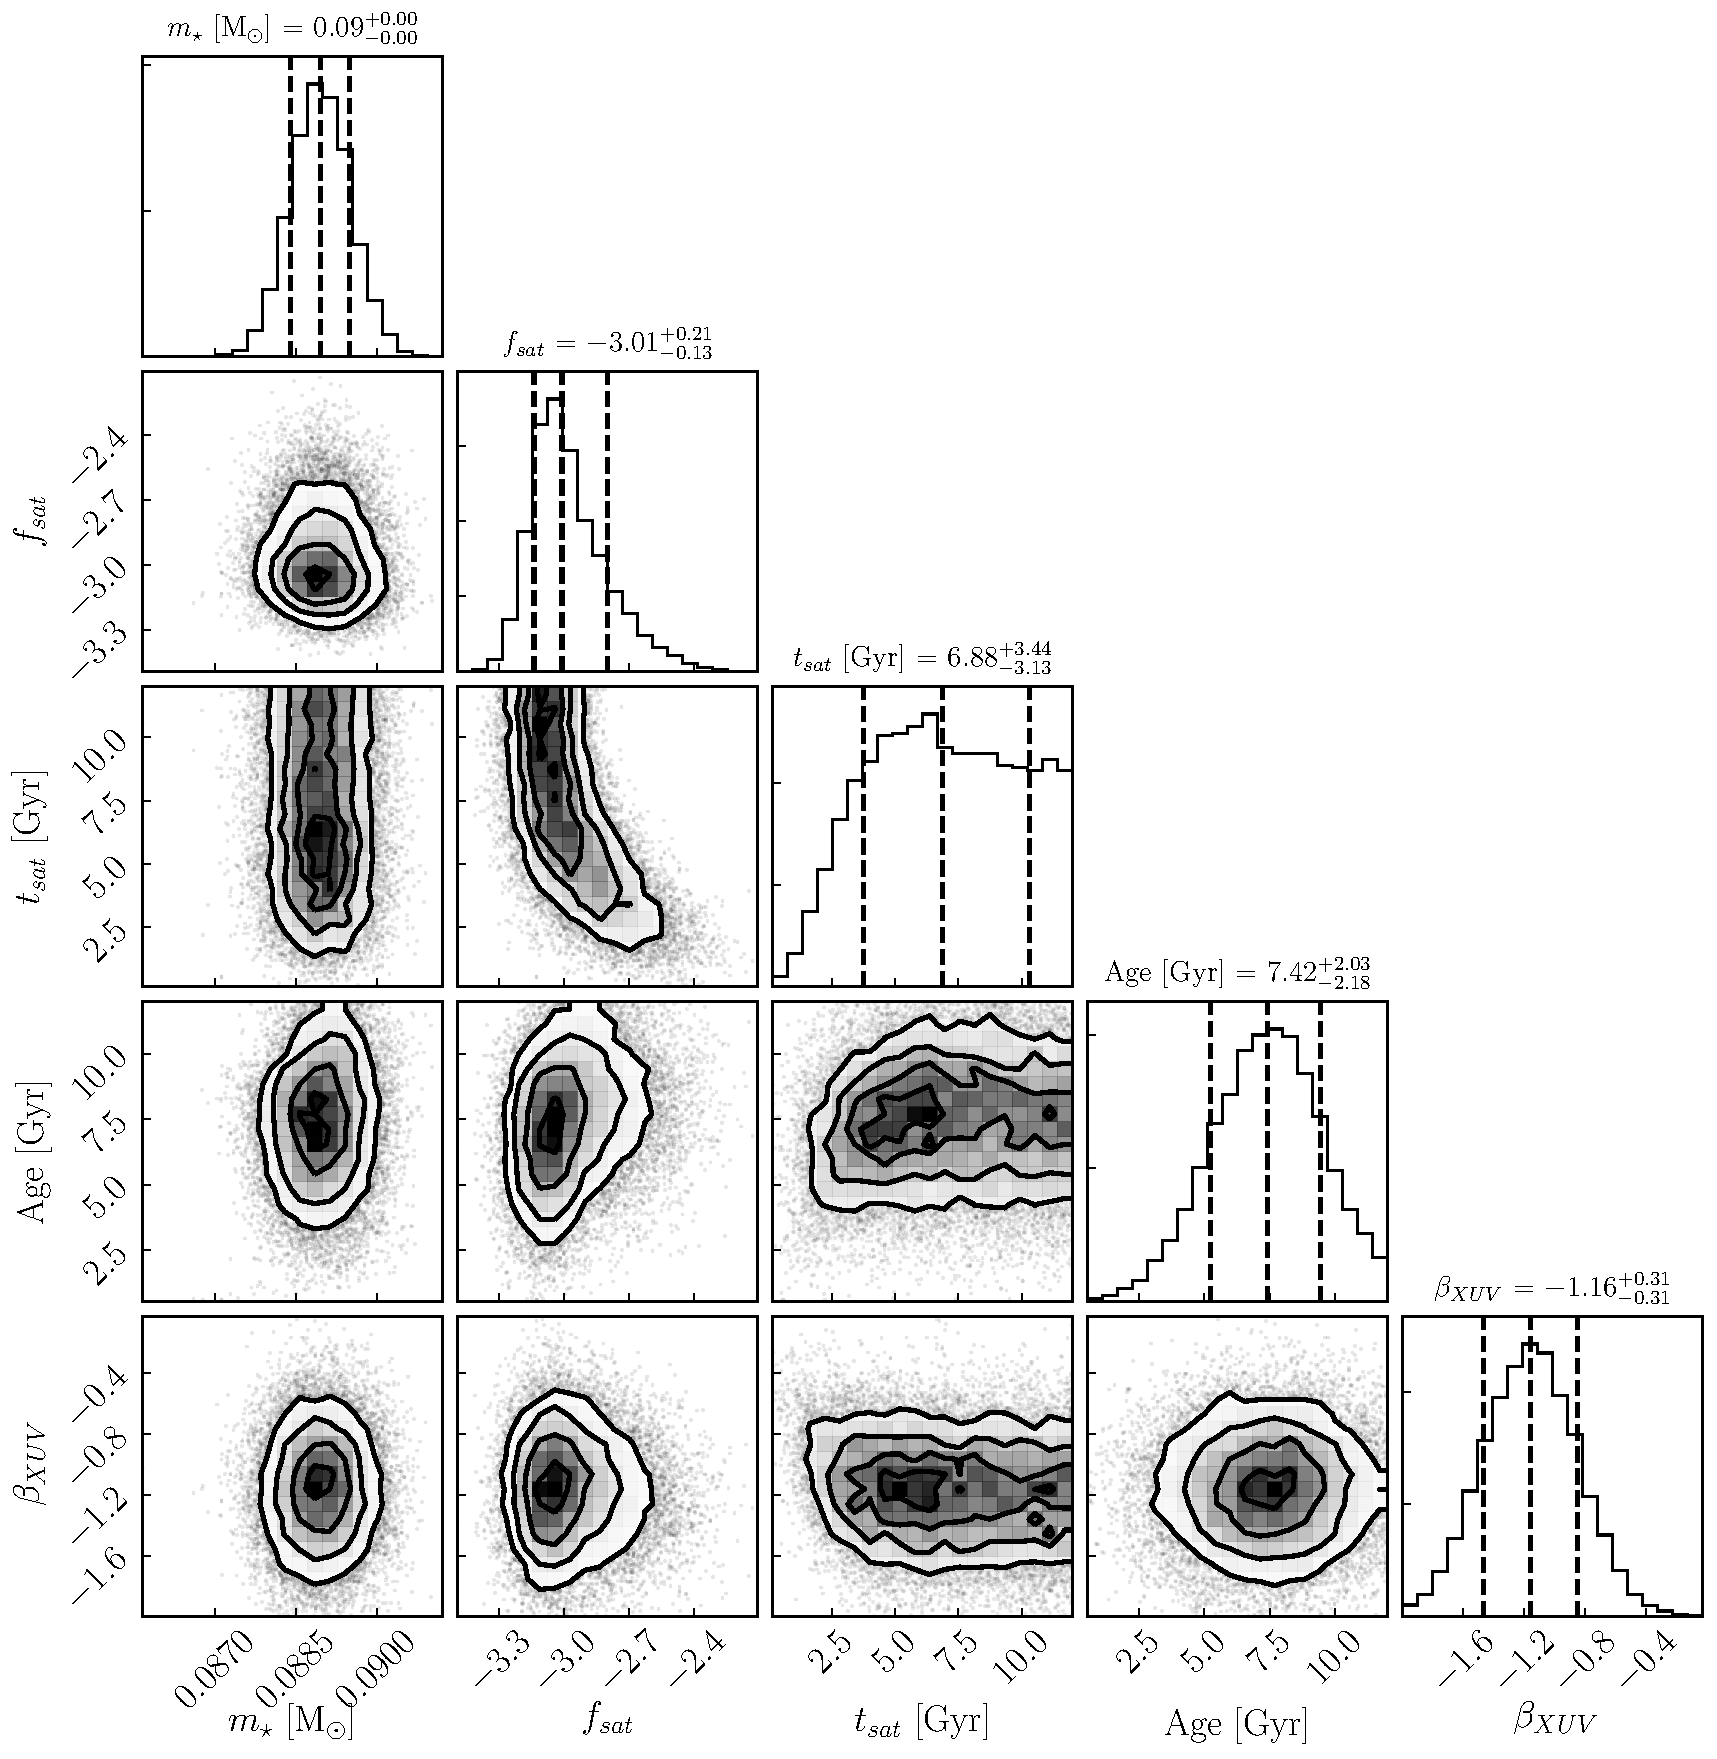
\includegraphics[width=0.75\textwidth]{../Analysis/Corner/trappist1Corner.pdf}
   \caption{Joint and marginal posterior probability distributions for the TRAPPIST-1 stellar parameters given in Eqn.~(\ref{eqn:state}) made using \texttt{corner} \citep{ForemanMackey2016}. The black vertical dashed lines on the marginalized distributions indicate the median values and lower and upper uncertainties from the 16th and 84th percentiles, respectively. From the posterior, we infer that there is a $43\%$ chance that TRAPPIST-1 is still in the saturated phase today, potentially driving significant volatile loss from its planets.}%
    \label{fig:corner}%
\end{figure*}

We constrain TRAPPIST-1's mass to $m_{\star} = 0.089 \pm{0.001}$ M$_{\odot}$, in a good agreement with and $6\times$ more precise than the value derived by \citet{vanGrootel2018}. Our marginalized age and $\beta_{XUV}$ posterior distributions reflect their prior distributions as for the former, $L_{bol}$ is not sufficient to further constrain TRAPPIST-1's age beyond our adopted prior since the luminosities of ultracool dwarfs do not significantly change during the main sequence \citep{Baraffe2015}. The posterior for $\beta_{XUV}$ does not vary from the prior because our XUV model is over-parameterized with 3 parameters to fit 2 observations, although all are motivated by empirical data and hence merit inclusion. Our model prefers to exploit the degeneracy between $f_{sat}$ and $t_{sat}$ to match TRAPPIST-1's observed $L_{XUV}$ in our MCMC instead of varying the slope of the unsaturated $L_{XUV}$ decay. Age and $\beta_{XUV}$ weakly correlate with $f_{sat}$, requiring a narrow spread of $f_{sat} \approx -3.05$ for young ages and steeper $\beta_{XUV}$, respectively. $\beta_{XUV}$ and $t_{sat}$ are uncorrelated, except at short $t_{sat}$ where steep $\beta_{XUV}$ are disfavored as this evolution would underpredict the observed $L_{XUV}$.

\subsection{TRAPPIST-1's Evolutionary History}

Here we consider plausible stellar evolutionary histories for TRAPPIST-1 by simulating 100 samples from the posterior distribution using \vplanet. We plot the evolution of TRAPPIST-1's $L_{bol}$, $L_{XUV}$, and radius in Fig.~\ref{fig:evol} and compare our models to the measured values. 

\begin{figure*}[t]
	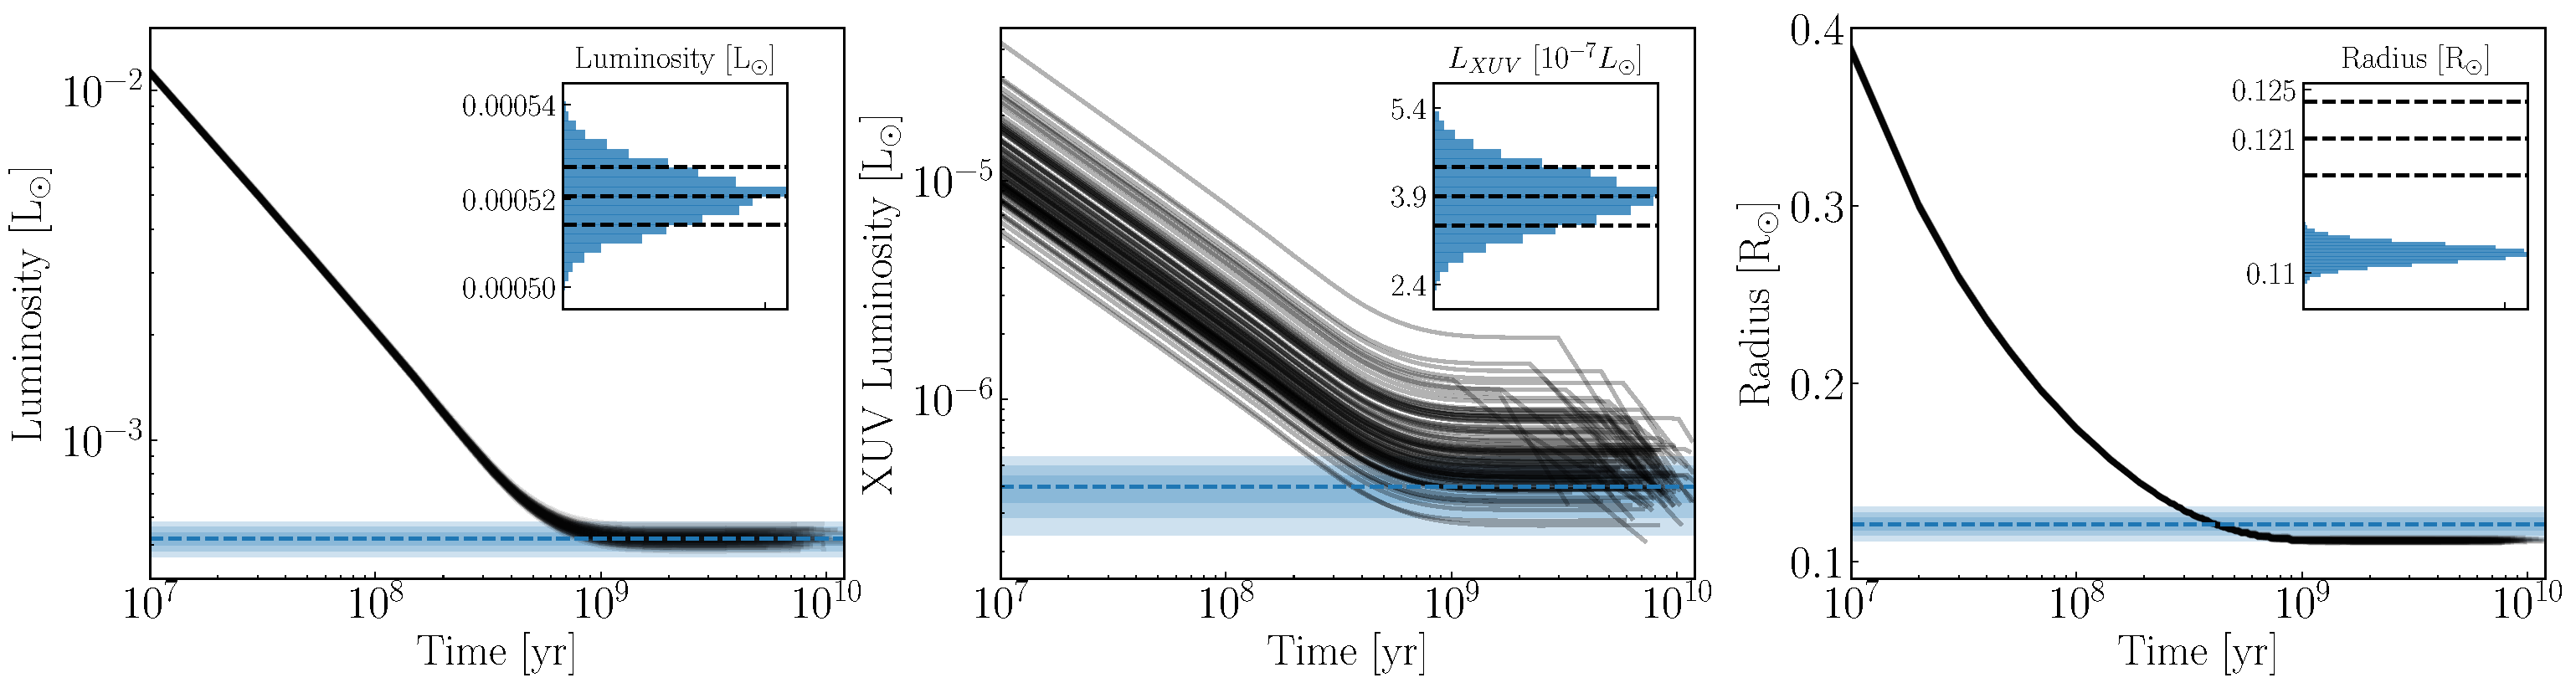
\includegraphics[width=\textwidth]{../Analysis/Evol/trappist1Evol.pdf}
   \caption{Plausible evolutionary histories of TRAPPIST-1's $L_{bol}$ (left), $L_{XUV}$ (center), and radius (right) using 100 samples drawn from the posterior distribution and simulated with \vplanet. In each panel, the blue shaded regions display the 1, 2, and 3 $\sigma$ uncertainties. The insets display the marginalized distributions (black) evaluated at the age of the system, with the blue dashed lines indicating the observed value and +/- 1 $\sigma$ uncertainties. The radius, $L_{bol}$, and $L_{XUV}$ constraints are adopted from \citet{vanGrootel2018} and \citet{Wheatley2017}, respectively.}%
    \label{fig:evol}%
\end{figure*}

TRAPPIST-1 remains saturated throughout its $1$ Gyr pre-main sequence, with both $L_{XUV}$ and $L_{bol}$ decreasing by a factor of ${\sim}40$ before stabilizing on the main sequence. TRAPPIST-1's radius likely shrank by roughly a factor of 4 along the pre-main sequence. We derive a present-day radius $R_{\star} = 0.112 \pm{0.001} \ R_{\odot}$ from the posterior distribution, a value that is ${\sim} 7\%$ smaller than the \citet{vanGrootel2018} constraint, $R_{\star} = 0.121 \pm {0.003} \ R_{\odot}$, that was computed from their inferred mass and TRAPPIST-1's density \citep{Delrez2018}. This difference arises from the likely underprediction of TRAPPIST-1's radius by the \citet{Baraffe2015} models, consistent with stellar evolution models often underestimating the radii of late M dwarfs \citep{Reid2005,Spada2013}. An alternate explanation to account for its inflated radius is that TRAPPIST-1 has super-solar metallicity \citep{Burgasser2017,vanGrootel2018}, but \citet{vanGrootel2018} found in their modeling that [Fe/H] = 0.4, a $4.5\sigma$ outlier, was required to reproduce TRAPPIST-1's density and radius. If we instead compute the radius from our marginalized stellar mass posterior distribution and the observed density \citep{Delrez2018}, we obtain $R_{\star} = 0.120 \pm{0.002} \ R_{\odot}$, in agreement with \citet{vanGrootel2018} who used the same procedure.

Since TRAPPIST-1 could still be saturated today, its planetary system has likely experienced a persistent extreme XUV environment. In Fig.~\ref{fig:fluxes}, we probe the distribution of XUV fluxes, $F_{XUV}$, derived from our posterior distributions for each TRAPPIST-1 planet when the system was 0.01, 0.1, and 1 Gyr old. We normalize these values by the $F_{XUV}$ received by Earth during the mean solar cycle \citep[$F_{XUV,\oplus} = 3.88$ erg s$^{-1}$cm$^{-2}$,][]{Ribas2005} and assume the planets remained near their current semi-major axes after migration in the natal protoplanetary disk halted \citep{Luger2017}. We infer that TRAPPIST-1b likely received extreme $F_{XUV}/F_{XUV, \oplus} \gsim 10^4$ during the early pre-main sequence before decaying to the present-day $F_{XUV}/F_{XUV, \oplus} \approx 10^3$, consistent with estimates from \citet{Wheatley2017}. The extended upper-tail of the $F_{XUV}$ distributions corresponds to the large $f_{sat}$ values permitted by the posterior distributions. The likely habitable zone planets, e, f, and g, similarly experienced severe XUV fluxes ranging from $F_{XUV}/F_{XUV, \oplus} \approx 10^2 - 10^{3.5}$ throughout the pre-main sequence. Even today, e, f, and g receive $F_{XUV}/F_{XUV, \oplus} \approx 10^2$, far in excess of the modern Earth, due to TRAPPIST-1's large present $L_{XUV}$, its extended saturated phase, and the close proximity of M dwarf HZ planets to their host star. These significant high energy fluxes likely drove an extended epoch of substantial atmospheric escape and water loss from the TRAPPIST-1 planets, potentially producing substantial abiotic O$_2$ atmospheres \citep{Luger2015,Bolmont2017,Bourrier2017a}.

\begin{figure}
	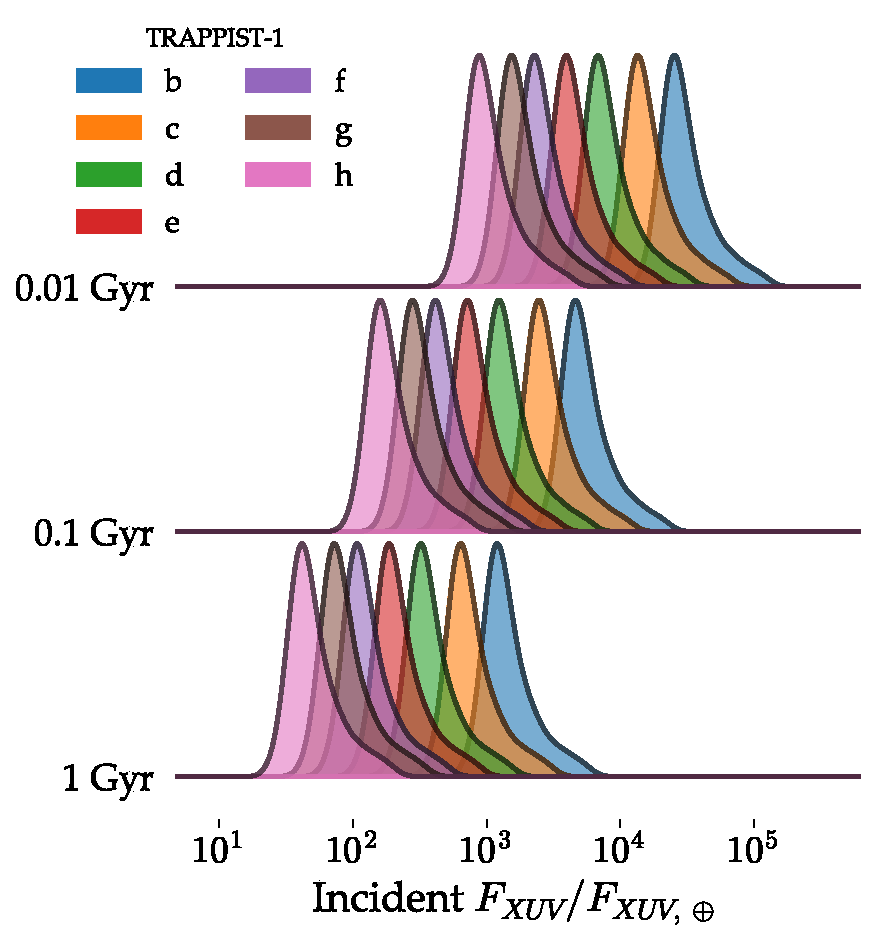
\includegraphics[width=\columnwidth]{../Analysis/Fluxes/fluxes.pdf}
   \caption{$F_{XUV}/F_{XUV,\oplus}$ for each TRAPPIST-1 planet derived from samples drawn from the posterior distribution and simulated using \vplanet when the system was 0.01, 0.1, and 1 Gyr old. The latter age corresponds to the approximate age at which TRAPPIST-1 entered the main sequence.}%
    \label{fig:fluxes}%
\end{figure}

%% approxposterior %%

\subsection{Comparison with \approxposterior} \label{sec:approx}

% Extra
%If using a slower model than ours, perhaps one that models stellar evolution by interpolating tracks over mass, age, and metallicity to additionally constrain [Fe/H], or if testing alternate models of $L_{XUV}$ evolution for model comparisons, the computational expense will grow, exacerbating this issue.

\begin{figure*}[t]
\centering
	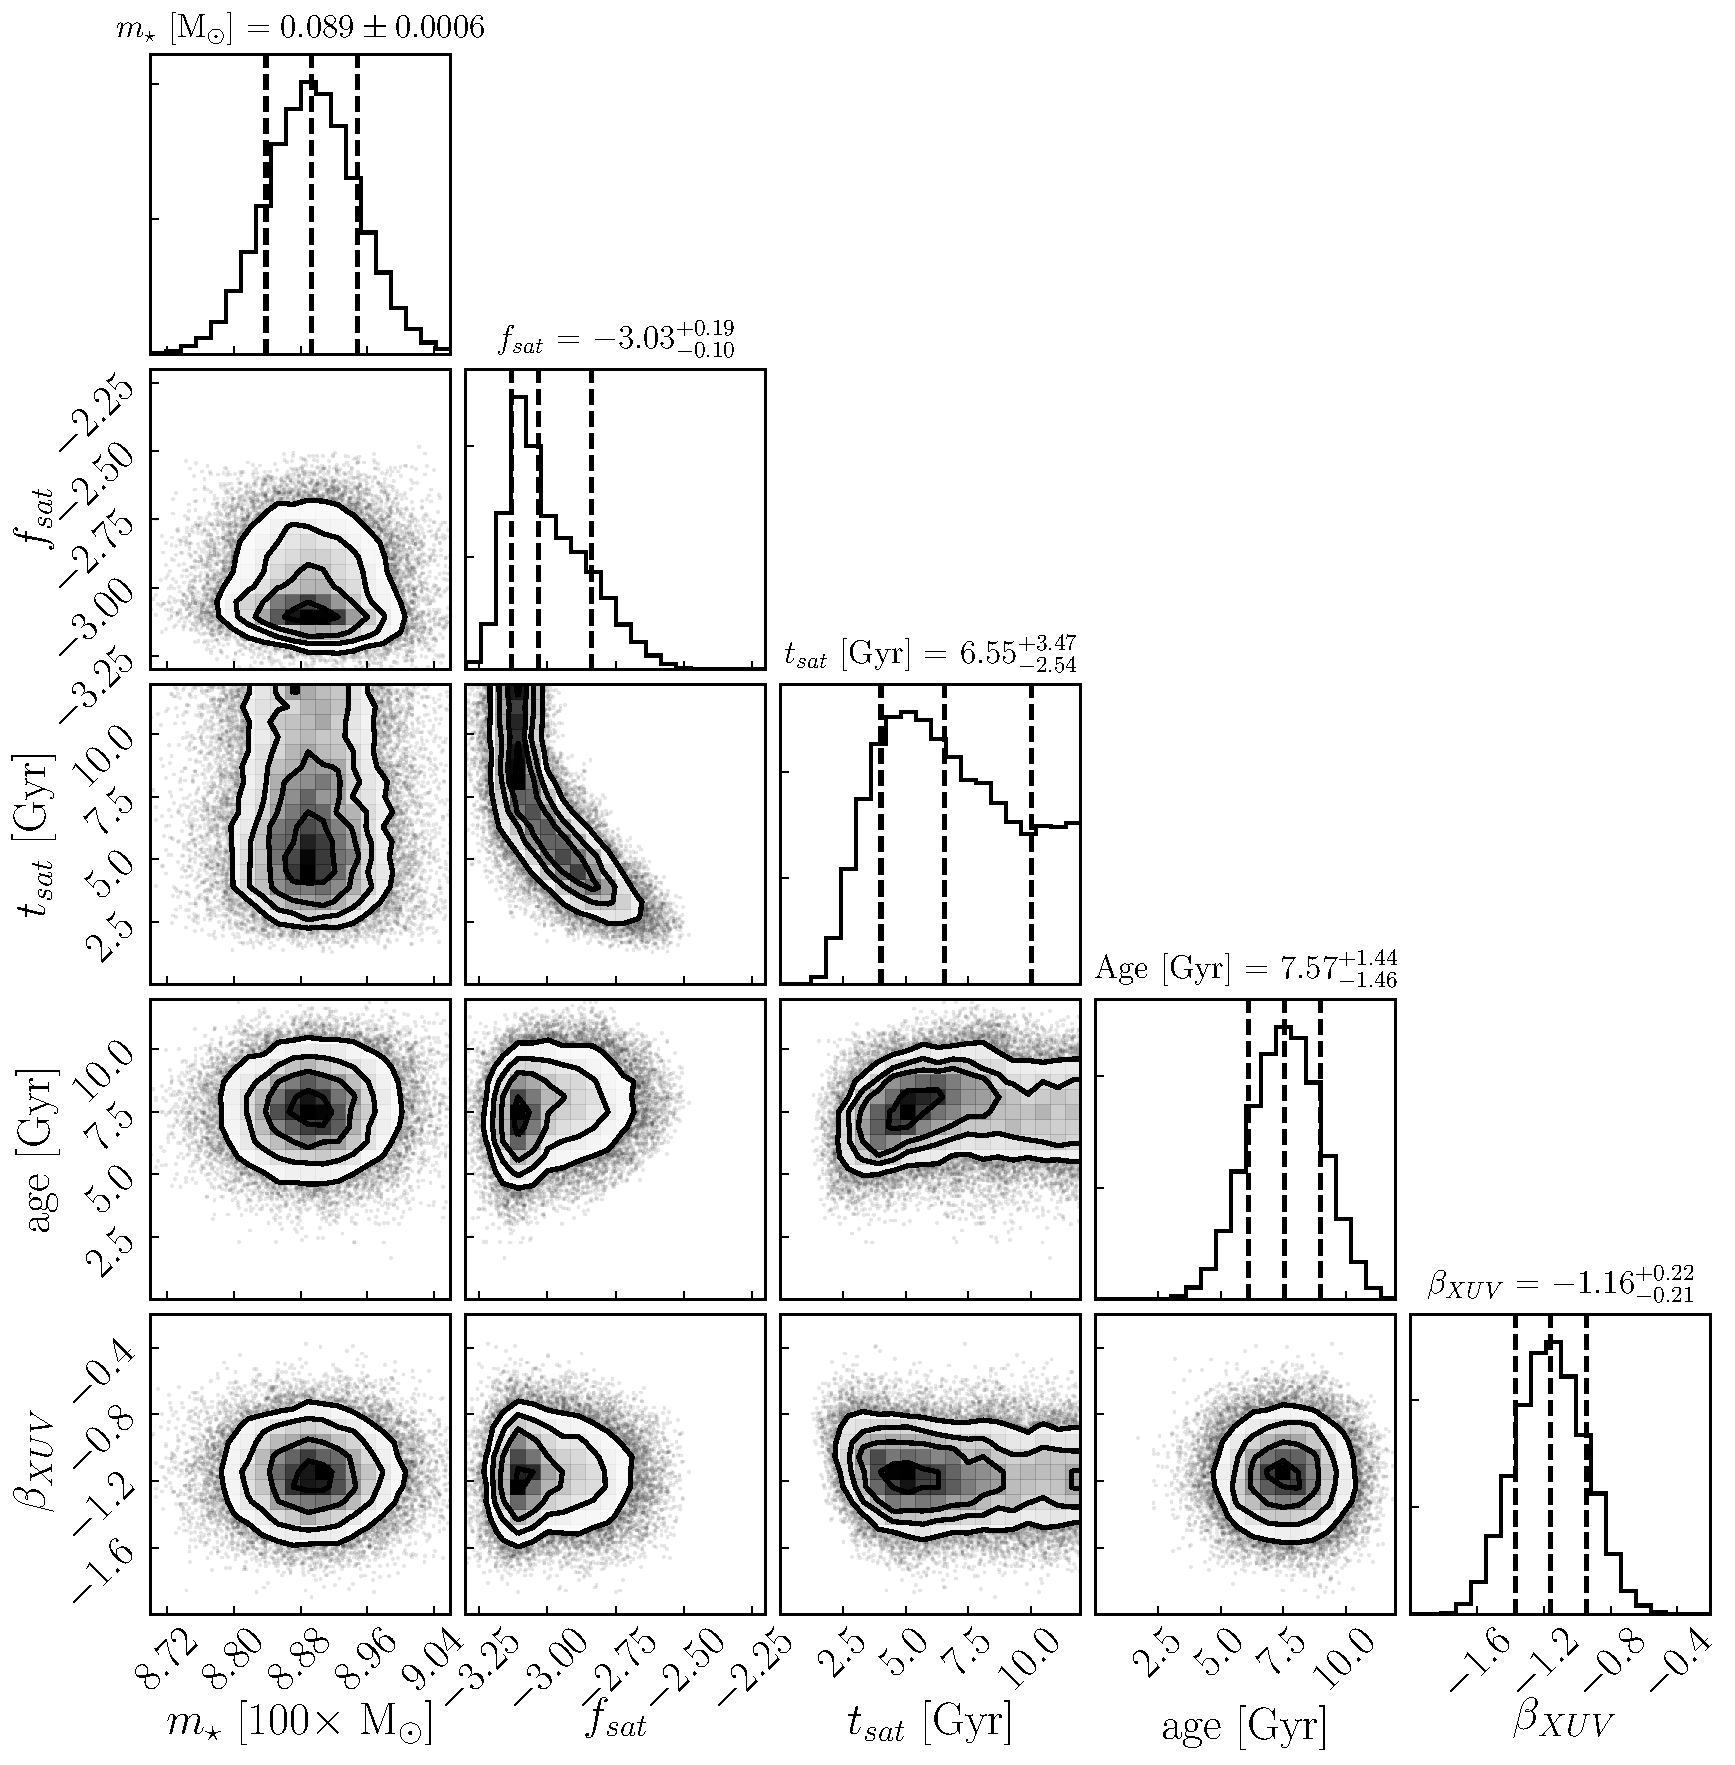
\includegraphics[width=0.75\textwidth]{../Analysis/Approx/apCorner.pdf}
   \caption{Same format as Fig.~\ref{fig:corner}, but derived by \approxposterior.}%
    \label{fig:approx}%
\end{figure*}

Here we compare the approximate posterior distribution derived using \approxposterior with our previous results (referred to as the fiducial MCMC). We display the approximate joint and marginalized posterior distributions in Fig.~\ref{fig:approx}. We find that \approxposterior requires only 11 core hours to derive the approximate posterior distribution, a factor of $330\times$ faster than our fiducial MCMC. \approxposterior also used $800\times$ fewer \vplanet simulations to build its training set than the ${\sim}10^6$ simulations ran by the fiducial MCMC for likelihood evaluations. This reduction in computational expense arises from \approxposterior's GP-based likelihood predictions only taking ${\sim}130\mu$s, compared to the much longer $10$~s per \vplanet simulation. Moreover, \approxposterior's efficient selection of the GP's training set focuses on high-likelihood regions to improve the GP's predictive ability in relevant regions of parameter space while minimizing the training set size. 

In Table~\ref{tab:constraints}, we list the marginalized constraints derived by both methods and find that both the median values and magnitude of the uncertainties are in good agreement. Furthermore as seen in Fig.~\ref{fig:approx}, \approxposterior recovers the same non-trivial correlations between model parameters seen in the fiducial MCMC posterior distribution. 

The posterior distribution derived by \approxposterior, however, is not an exact match. \approxposterior underestimates the magnitude of both the age and $\beta_{XUV}$ uncertainties by ${\sim}30\%$ and predicts that there is a $39\%$ chance that TRAPPIST-1 is still saturated today, $9\%$ smaller than the fiducial MCMC-derived value. Our experiment demonstrates that \approxposterior can be used to derive accurate approximations to the posterior probability distributions of the parameters that control stellar XUV evolution in late M dwarfs, but significantly faster than traditional MCMC methods.

\begin{deluxetable}{lcc}
\caption{Parameter Constraints} \label{tab:constraints}
\tabletypesize{\small}
\tablewidth{0pt}
\tablehead{
\colhead{Parameter [units]} & \colhead{\vplanet MCMC} & \colhead{\approxposterior MCMC}
}
\startdata
$m_\star$ [$M_{\odot}$] & $0.089 \pm{0.001}$ & $0.089 \pm{0.001}$ \\  
$f_{sat}$ & $-3.05^{+0.24}_{-0.10}$ & $-3.03^{+0.20}_{-0.10}$,  \\
$t_{sat}$ [Gyr] & $6.85^{+3.43}_{-3.15}$ & $6.62^{+3.56}_{-2.56}$ \\
age [Gyr] & $7.44^{+2.04}_{-2.13}$ & $7.54^{+1.43}_{-1.51}$ \\
$\beta_{XUV}$ & $-1.16^{+0.31}_{-0.30}$ & $-1.16^{+0.21}_{-0.21}$ \\
P$(\mathrm{saturated})$ & $0.43$ & $0.39$ \\
\enddata \vspace*{0.1in}
\tablecomments{Best fit values and uncertainties are derived using the medians, $16^{th}$, and $84^{th}$ percentiles from the marginalized posterior distributions, respectively.}
\end{deluxetable}

%% Discussion %%

\section{Discussion and Conclusions} \label{sec:discussion}

Here, we used MCMC to derive probabilistic constraints for TRAPPIST-1's stellar and $L_{XUV}$ evolution to characterize the evolving XUV environment of its planetary system. We inferred that TRAPPIST-1 likely maintained high $L_{XUV}/L_{bol} \approx 10^{-3}$ throughout its lifetime, with a $43\%$ chance that TRAPPIST-1 is still in the saturated regime today. Our results indicate that ultracool dwarfs can sustain large $L_{XUV}$ in the saturated regime for Gyrs, consistent with activity lifetimes of late M dwarfs \citep{West2008}. Our choice of prior distributions strongly impact our results as our inference hinges on only two measured properties of TRAPPIST-1, $L_{XUV}$ and $L_{bol}$. To mitigate this effect, we consulted previous studies and empirical observations of the activity evolution of late M dwarfs to construct realistic prior distributions.

The TRAPPIST-1 planets likely experienced significant XUV fluxes during the pre-main sequence, potentially driving extreme atmospheric erosion and water loss \citep{Bolmont2017,Bourrier2017a}. The high-energy fluxes incident on the inner-most planets throughout this phase were probably large enough for atmospheric mass loss to be recombination-limited ($F_{UV} \gsim 10^4$ g s$^{-1}$ cm$^{-2}$) and scale as $\dot{m} \sim F_{XUV}^{0.6}$ \citep{MurrayClay2009}, as opposed to the oft-assumed energy-limited escape \citep[$\dot{m} \sim F_{XUV}$,][]{Watson1981,Lammer2003}, potentially inhibiting volatile loss. If the TRAPPIST-1 planets did lose significant amounts of water as our estimates suggest, they must have formed with a large initial volatile inventory to account for their observed low densities \citep{Grimm2018}.

We demonstrated that the machine learning Python package, \approxposterior \citep{FlemingVanderPlas2018}, can efficiently compute an approximation to the posterior distribution using an adaptive GP-based method, requiring $800\times$ fewer \vplanet simulations and a factor of $330\times$ less core hours than traditional MCMC approaches for this application. The posterior distributions derived by \approxposterior accurately reproduced the non-trivial parameter correlations and best-fit values uncovered by our fiducial MCMC analysis. The agreement is not perfect, however as \approxposterior underestimated the magnitude of the uncertainties of two parameters by ${\sim}30\%$.  

Finally, we note that our methodology constrains parameters that describe the long-term XUV evolution of the star, conditioned on measurements. In principle, this approach can be extended to obtain evolutionary histories of planetary systems in general.  For example, in Figures~\ref{fig:evol} and \ref{fig:fluxes}, we examined the long-term evolution of TRAPPIST-1 and the evolving XUV fluxes received by its planetary system, respectively, with samples drawn from the posterior distribution. Future research can combine those results with additional physical effects, e.g. water loss or tidal dissipation, to build a probabilistic model for the long-term evolution of the planetary system, given our model for the underlying physics, to characterize its present state. While simulating additional physical effects will inevitably increase the computational expense, we have demonstrated that \approxposterior can enable such efforts and provide insight into the histories of stars and their planets.

% extra
% Applying these methods to other M dwarfs, however, requires measuring their current $L_{X}$ or $L_{XUV}$, a difficult task given that most M and ultracool dwarfs are faint and that much of the stellar EUV radiation is absorbed by neutral interstellar hydrogen \citep{Airapetian2019}. These quantities, however, can be reconstructed via empirical scaling relations \citep[e.g.][]{Linsky2014}. 
% The accuracy and massive reduction in compute time afforded by \approxposterior enables our analysis to scale to a larger sample of late M dwarfs to constrain their XUV histories.


%% ACKNOWLEDGEMENTS %%
\acknowledgments
This work was facilitated though the use of advanced computational, storage, and networking infrastructure provided by the Hyak supercomputer system and funded by the Student Technology Fund at the University of Washington. DPF was supported by NASA Headquarters under the NASA Earth and Space Science Fellowship Program - Grant 80NSSC17K0482.  This work was supported by the NASA Astrobiology Program Grant Number 80NSSC18K0829 and benefited from participation in the NASA Nexus for Exoplanet Systems Science research coordination network.

%% SOFTWARE %%
\software{\approxposterior: \citet{FlemingVanderPlas2018}, \texttt{corner}: \citet{ForemanMackey2016}, \texttt{emcee}: \citet{ForemanMackey2013}, \vplanet: \citet{Barnes2019}} 

%% BIBLIOGRAPHY %%

\bibliography{trappist}

% End of file
\end{document}